% TODO bibliography?
\documentclass{beamer}
\usepackage{animate}
\usepackage[english]{babel}
\usepackage[utf8]{inputenc}
\usepackage{algorithm}
\usepackage[noend]{algpseudocode}
\usepackage{graphics}
\usepackage[final]{pdfpages}
\usepackage[font=small, skip=0pt]{caption}
\setbeamertemplate{frametitle continuation}[from second][(contd.)]
\setbeamertemplate{itemize items}{--}
\beamertemplatenavigationsymbolsempty

\title{Proximal Policy Optimization with Dynamic Clipping}
\author{Student: Rishikesh Vaishnav\\Mentor: Sicun Gao}

\begin{document}
\captionsetup{labelformat=empty, font=footnotesize}
\renewcommand{\thealgorithm}{}
\maketitle
\begin{frame}[noframenumbering, allowframebreaks]{Background}
    Reinforcement Learning
    \begin{itemize}
        \item A set of algorithms that seek to replicate behavioral learning.
        \item Basic vocabulary:
        \begin{itemize}
            \item \textbf{Environment}: a general setting with changeable
                parameters in which actions can be performed that affect these
                parameters
            \item \textbf{State} (denoted $s$): a specific configuration (i.e. ``snapshot'')
                of an environment
            \item \textbf{Agent}: an entity that learns to accomplish a task in
                a specific evironment
            \item \textbf{Action} (denoted $a$): a decision made by the agent that is intended
                to affect subsequent states
            \item \textbf{Episode}: a sequence of states and actions in an
                environment
            \item \textbf{Reward} (denoted $r$): a number associated with a state-action pair
        \end{itemize}
        \item Overall goal: train an agent that picks actions such that the sum
            of the rewards over an episode is maximimized.
        \framebreak
        \item Example: cart-pole demo
            \animategraphics[autoplay,loop,width=\linewidth]{25}
                {cartpole_ex/coalesced/cartpole_ex-}{0}{372}
        % NOTE explain how each of the previous terms manifests itself in this
        % example
    \end{itemize}
    \framebreak
    Policy Gradient Methods
    \begin{itemize}
        \item An agent can be provided with a \textbf{policy}, usually denoted
            $\pi$, that completely specifies the probabilty distribution of the
            action that should be taken at any particular state.
        \item $\pi$ is parameterized by some vector $\theta$ and can be any
            function of a state $s_t$.
        % NOTE mention that this is usually done using neural networks, in
        % which context theta is the vector of weights
        \item The task of the agent is to learn $\theta$.
    \end{itemize}
    \framebreak
    Generic Policy Gradient Algorithm
    \begin{algorithm}[H]
        \caption{Generic Policy Gradient}
        \begin{algorithmic}
            \State Initialize $\theta$ arbitrarily
            \While{True}\Comment{loop forever}
                \State $\theta_{old} \gets \theta$
                \State $rollout \gets (s, a, r)$ from multiple
                $\pi_{\theta}$ episodes 
                % NOTE explain what a rollout is and what (s, a, r) are
                \State Set $\theta$ to maximize the loss function $L(rollout,
                \theta, \theta_{old})$
            \EndWhile
        \end{algorithmic}
    \end{algorithm}
    \framebreak
    Trust Region Policy Optimization (TRPO)
    \begin{itemize}
        \item The theory behind TRPO suggests using the loss function:
        \begin{align*}
            L_{\theta_{old}}(\theta) 
            - CD_{KL}^{max}(\theta, \theta_{old})
        \end{align*}
        where $C$ is a constant and
        \begin{align*}
            L_{\theta_{old}}(\theta) &=
            \mathbb{E}_t \left[ 
            \frac
            {\pi_{\theta}(a_t | s_t)}
            {\pi_{\theta_{old}} (a_t | s_t)}
            A_t
            \right]
        \end{align*}.
        \item Using this loss function guarantees monotonic improvement.
        % NOTE this requires that L is precisely calculated and that the
        % function is maximized (both impossible in practice)
        % NOTE the specifics of this equation are not important for our
        % discussion - what is important to notice is the tradeoff between the
        % surrogate loss and the penalty
        \item Using the penalty term $CD_{KL}^{max}(\theta, \theta_{old})$
        leads to small step sizes in practice, so TRPO uses a hard constraint
        on the KL divergence.
    \end{itemize}
    \framebreak
    Proximal Policy Optimization (PPO)
    \begin{itemize}
        \item PPO uses a loss function that is an approximation to the TRPO
            loss:
        \begin{align*}
            L^{CLIP}(\theta) &= \mathbb{E}\left[ 
            \min\left(r_tA_t, \text{clip}
            (r_t, 1 - \epsilon, 1 + \epsilon)A_t\right)
            \right]
        \end{align*}
        where 
        $r_t(\theta) = 
        \frac
        {\pi_{\theta}(a_t | s_t)}
        {\pi_{\theta_{old}} (a_t | s_t)}$.
        % NOTE note that first term and TRPO L function are identical
        \framebreak
        \item Resultant clipping behavior:\\
        \begin{center}
            \begin{figure}[H]
                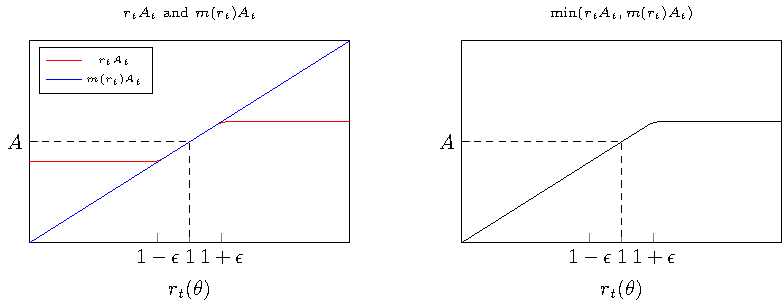
\includegraphics[page=1, scale=0.6]{clip_graph/clip_graph}
                \caption{Case $A > 0$}
            \end{figure}
            \begin{figure}[H]
                \includegraphics[page=2, scale=0.6]{clip_graph/clip_graph}
                \caption{Case $A > 0$}
            \end{figure}
        \end{center}
        % NOTE we can think of the clipped-off area as a replacement for the
        % penalty term in the original TRPO
        \framebreak
        \item Research question: how can we more precisely control penalties 
            introduced through the clipping objective?
    \end{itemize}
\end{frame}

\begin{frame}[noframenumbering, allowframebreaks]{Potential Shortcoming of PPO}
    \begin{itemize}
        \item We can separate the loss into its positive and negative
            components:
        \begin{align*}
            L^{CLIP}(\theta) &= \mathbb{E}_t\left[ 
            \min\left(r_tA_t, \text{clip}
            (r_t, 1 - \epsilon, 1 + \epsilon)A_t\right)\right]\\
            &= \mathbb{E}_t\left[ 
            \begin{cases}
                \min\left(r_t, \text{clip}
                (r_t, 1 + \epsilon)\right)A_t & A_t > 0\\
                \max\left(r_t, \text{clip}
                (r_t, 1 - \epsilon)\right)A_t & A_t < 0
            \end{cases}\right]
        \end{align*}
        \item Let:
        \begin{align*}
            r_{t, CLIP}^+ &= 
            \min\left(r_t, \text{clip}
            (r_t, 1 + \epsilon)\right)\\
            r_{t, CLIP}^- &= 
            \max\left(r_t, \text{clip}
            (r_t, 1 - \epsilon)\right)
        \end{align*}
        \item We know that:
        \begin{align*}
            \mathbb{E}_t[r_{t, CLIP}^+] &< 1\\
            \mathbb{E}_t[r_{t, CLIP}^-] &> 1\\
        \end{align*}\\

        \framebreak
        \item Now, we can define the ``expected penalty contributions'' of
            positive and negative advantages:
        \begin{align*}
            1 - \mathbb{E}_t[r_{t, CLIP}^+]
        \end{align*}
        and
        \begin{align*}
            \mathbb{E}_t[r_{t, CLIP}^-] - 1
        \end{align*}
        \item Because $r_t$ and $A_t$ are not independent, these expected
            penalty contributions do not suggest actual penalty contributions.
        \item However, they can indicate inherent imbalances in the system.
    \end{itemize}
    \framebreak
    Conceptual Example
    \begin{itemize}
        \item Consider a typical example in reinforcement learning where:
            \begin{itemize}
                \item We have an agent using a continuous action
                    space (continuous control).
                \item The policy is encoded by a gaussian with state-dependent
                    means but constant standard deviation.
                % NOTE explain this carefully
            \end{itemize}
    \end{itemize}
    \framebreak
    What happens as we learn?\\
    % NOTE note that we are restrincting our view to a particular state, but
    % this happens in general across all states
    \begin{center}
        \animategraphics[scale=0.5,autoplay,loop]{15}{discrepancy}{}{}
    \end{center}
    %NOTE mention increasing discrepancy
    \framebreak
    \begin{itemize}
        \item The discrepancy between positive and negative penalty
            contributions is unintentional and highly dependent on the shape of
            the distribution.
        \item The goal of this project is to investigate the effects of
            controlling this discrepancy directly.
    \end{itemize}<++>
\end{frame}

\begin{frame}[noframenumbering, allowframebreaks]{Idea}
\end{frame}

\begin{frame}[noframenumbering, allowframebreaks]{Results}
\end{frame}

\begin{frame}[noframenumbering, allowframebreaks]{Future Directions}
\end{frame}

\end{document}
